\documentclass{book}
\usepackage{commeunjeustyle}

\begin{document}

\chapter*{Structures algébriques}%label=ch_structures_algebriques
\begin{Texte}%label=introduction
L'enfant apprend d'abord : 
\begin{itemize}
\item à \impo{compter} le nombre d'objets en itérant l'ajout d'une unité à partir de 0 c'est à dire en construisant l'ensemble $\N$  avec l'opération "suivant"
\begin{center}
\begin{tikzpicture}
\draw[color=colorprop] (0,0) rectangle (1,1);
\node at (0.5,-0.3){$0$};
\draw[color=colorprop] (1.5,0) rectangle (2.5,1);
\draw[color=colordef] (2,0.5) circle (0.15);
\node at (2,-0.3){$1$};
\draw[color=colorprop] (3,0) rectangle (4,1);
\draw[color=colordef] (3.3,0.2) circle (0.15);
\draw[color=colordef] (3.7,0.7) circle (0.15);
\node at (3.5,-0.3){$2$};
\draw[color=colorprop] (4.5,0) rectangle (5.5,1);
\draw[color=colordef] (4.8,0.75) circle (0.15);
\draw[color=colordef] (4.7,0.2) circle (0.15);
\draw[color=colordef] (5.3,0.5) circle (0.15);
\node at (5,-0.3){$3$};
\end{tikzpicture}\\
Désignation à l'aide d'un nombre de la quantité de cercles dans le carré à partir de $0$
\end{center}
\item à \impo{ordonner} en comparant des quantités c'est à munir d'une structure d'ordre à l'ensemble $\N$ 
\begin{center}
\begin{tikzpicture}
\draw[color=colorprop] (1.5,0) rectangle (2.5,1);
\draw[color=colordef] (2,0.5) circle (0.15);
\node at (3,0.5){$\leq$};
\draw[color=colorprop] (3.5,0) rectangle (4.5,1);
\draw[color=colordef] (3.8,0.75) circle (0.15);
\draw[color=colordef] (3.7,0.2) circle (0.15);
\draw[color=colordef] (4.3,0.5) circle (0.15);
\end{tikzpicture}\\
Comparaison de deux quantités de cercles 
\end{center}
\end{itemize}
Puis il commence :
\begin{itemize}
\item  à \impo{additionner} les nombres en opérant des regroupements.
\begin{center}
\begin{tikzpicture}
\draw[color=colorprop,fill=colorprop!20] (0,0) rectangle (1,1);
\draw[color=colorprop,fill=colorprop!20] (1,0) rectangle (2,1);
\draw[color=colorprop,fill=colorprop!20] (2,0) rectangle (3,1);
\node at (1,-0.5){$3$};
\node at (3.5,0.5){$+$};
\node at (3.5,-0.5){$+$};
\draw[color=colordef,fill=colordef!20] (4,0) rectangle (5,1);
\draw[color=colordef,fill=colordef!20] (5,0) rectangle (6,1);
\node at (5,-0.5){$2$};
\node at (6.5,0.5){$=$};
\node at (6.5,-0.5){$=$};
\draw[color=colorprop,fill=colorprop!20] (7,0) rectangle (8,1);
\draw[color=colorprop,fill=colorprop!20] (8,0) rectangle (9,1);
\draw[color=colorprop,fill=colorprop!20] (9,0) rectangle (10,1);
\draw[color=colordef,fill=colordef!20] (10,0) rectangle (11,1);
\draw[color=colordef,fill=colordef!20] (11,0) rectangle (12,1);
\node at (9.5,-0.5){$5$};
\end{tikzpicture}\\
Regroupement de cubes pour additionner
\end{center}
\item  à \impo{multiplier} les nombres en opérant une addition itérée.
\begin{center}
\begin{tikzpicture}
\draw[color=colorprop,fill=colorprop!20] (-10,0) rectangle (-9,1);
\draw[color=colorprop,fill=colorprop!20] (-10,1) rectangle (-9,2);
\node[scale=2] at (-8.5,1){$+$};
\draw[color=colorprop,fill=colorprop!20] (-8,0) rectangle (-7,1);
\draw[color=colorprop,fill=colorprop!20] (-8,1) rectangle (-7,2);
\node[scale=2] at (-6.5,1){$+$};
\draw[color=colorprop,fill=colorprop!20] (-6,0) rectangle (-5,1);
\draw[color=colorprop,fill=colorprop!20] (-6,1) rectangle (-5,2);
\node[scale=2] at (-4.5,1){$=$};
\draw[color=colorprop,fill=colorprop!20] (-4,0) rectangle (-3,1);
\draw[color=colorprop,fill=colorprop!20] (-3,0) rectangle (-2,1);
\draw[color=colorprop,fill=colorprop!20] (-2,0) rectangle (-1,1);
\draw[color=colorprop,fill=colorprop!20] (-4,1) rectangle (-3,2);
\draw[color=colorprop,fill=colorprop!20] (-3,1) rectangle (-2,2);
\draw[color=colorprop,fill=colorprop!20] (-2,1) rectangle (-1,2);
\node at (-5,-0.5) {$\overbrace{2+2+2}^{3 \text{ fois}}\quad=\quad 3\times 2$};
\end{tikzpicture}\\
Regroupement itéré de cubes pour multiplier
\end{center}
 \end{itemize}
Ensuite il s'intéresse aux propriétés des opérations :
\begin{itemize}
 \item \impo{associativité} de l'addition $(a+b)+c=a+(b+c)$ et de la multiplication $(a\times b)\times c=a\times(b \times c)$
\begin{center}
\begin{tikzpicture}[scale=0.75]
\node[scale=2] at (-0.2,0.5){$($};
\draw[color=colorprop,fill=colorprop!20] (0,0) rectangle (1,1);
\draw[color=colorprop,fill=colorprop!20] (1,0) rectangle (2,1);
\draw[color=colorprop,fill=colorprop!20] (2,0) rectangle (3,1);
\node[scale=2] at (3.5,0.5){$+$};
\draw[color=colordef,fill=colordef!20] (4,0) rectangle (5,1);
\draw[color=colordef,fill=colordef!20] (5,0) rectangle (6,1);
\node[scale=2] at (6.5,0.5){$)+$};
\draw[color=green,fill=green!20] (7,0) rectangle (8,1);
\node[scale=2] at (8.5,0.5){$=$};
\draw[color=colorprop,fill=colorprop!20] (9,0) rectangle (10,1);
\draw[color=colorprop,fill=colorprop!20] (10,0) rectangle (11,1);
\draw[color=colorprop,fill=colorprop!20] (11,0) rectangle (12,1);
\draw[color=colordef,fill=colordef!20] (12,0) rectangle (13,1);
\draw[color=colordef,fill=colordef!20] (13,0) rectangle (14,1);
\node[scale=2] at (14.5,0.5){$+$};
\draw[color=green,fill=green!20] (15,0) rectangle (16,1);
\node[scale=2] at (16.5,0.5){$=$};
\draw[color=colorprop,fill=colorprop!20] (17,0) rectangle (18,1);
\draw[color=colorprop,fill=colorprop!20] (18,0) rectangle (19,1);
\draw[color=colorprop,fill=colorprop!20] (19,0) rectangle (20,1);
\draw[color=colordef,fill=colordef!20] (20,0) rectangle (21,1);
\draw[color=colordef,fill=colordef!20] (21,0) rectangle (22,1);
\draw[color=green,fill=green!20] (22,0) rectangle (23,1);


\draw[color=colorprop,fill=colorprop!20] (0,-1) rectangle (1,-2);
\draw[color=colorprop,fill=colorprop!20] (1,-1) rectangle (2,-2);
\draw[color=colorprop,fill=colorprop!20] (2,-1) rectangle (3,-2);
\draw[color=colordef,fill=colordef!20] (3,-1) rectangle (4,-2);
\draw[color=colordef,fill=colordef!20] (4,-1) rectangle (5,-2);
\draw[color=green,fill=green!20] (5,-1) rectangle (6,-2);
\node[scale=2] at (6.5,-1.5){$=$};
\draw[color=colorprop,fill=colorprop!20] (7,-1) rectangle (8,-2);
\draw[color=colorprop,fill=colorprop!20] (8,-1) rectangle (9,-2);
\draw[color=colorprop,fill=colorprop!20] (9,-1) rectangle (10,-2);
\node[scale=2] at (10.5,-1.5){$+$};
\draw[color=colordef,fill=colordef!20] (11,-1) rectangle (12,-2);
\draw[color=colordef,fill=colordef!20] (12,-1) rectangle (13,-2);
\draw[color=green,fill=green!20] (13,-1) rectangle (14,-2);
\node[scale=2] at (14.5,-1.5){$=$};
\draw[color=colorprop,fill=colorprop!20] (15,-1) rectangle (16,-2);
\draw[color=colorprop,fill=colorprop!20] (16,-1) rectangle (17,-2);
\draw[color=colorprop,fill=colorprop!20] (17,-1) rectangle (18,-2);
\node[scale=2] at (18.5,-1.5){$+($};
\draw[color=colordef,fill=colordef!20] (19,-1) rectangle (20,-2);
\draw[color=colordef,fill=colordef!20] (20,-1) rectangle (21,-2);
\node[scale=2] at (21.5,-1.5){$+$};
\draw[color=green,fill=green!20] (22,-1) rectangle (23,-2);
\node[scale=2] at (23.2,-1.5){$)$};
\end{tikzpicture}\\
Démonstration géométrique élémentaire de l'associativité  de l'addition
\end{center}
\item \impo{commutativité} de l'addition $a+b=b+a$ et de la multiplication $a\times b=b\times a$
\begin{center}
\begin{tikzpicture}
\draw[color=colorprop,fill=colorprop!20] (0,0) rectangle (1,1);
\draw[color=colorprop,fill=colorprop!20] (1,0) rectangle (2,1);
\draw[color=colorprop,fill=colorprop!20] (2,0) rectangle (3,1);
\draw[color=colordef,fill=colordef!20] (0,1) rectangle (1,2);
\draw[color=colordef,fill=colordef!20] (1,1) rectangle (2,2);
\draw[color=colordef,fill=colordef!20] (2,1) rectangle (3,2);
\node[scale=2] at (-0.5,1){$=$};
\draw[color=colorprop,fill=colorprop!20] (-4,0) rectangle (-3,1);
\draw[color=colordef,fill=colordef!20] (-3,0) rectangle (-2,1);
\draw[color=green,fill=green!20] (-2,0) rectangle (-1,1);
\draw[color=colorprop,fill=colorprop!20] (-4,1) rectangle (-3,2);
\draw[color=colordef,fill=colordef!20] (-3,1) rectangle (-2,2);
\draw[color=green,fill=green!20] (-2,1) rectangle (-1,2);
\node at (-1,-0.5) {$\overbrace{a}^{\text{Nombre de colonnes}}\times \overbrace{b}^{\text{Nombre de cubes par colonne}}\quad=\quad \overbrace{b}^{\text{Nombre de lignes}}\times \overbrace{a}^{\text{Nombre de cubes par ligne}}$};
\end{tikzpicture}\\
Démonstration géométrique élémentaire de la commutativité  de la multiplication
\end{center}
\item \impo{distributivité} de la multiplication sur l'addition $a\times (b+c)=(a\times b)+(a\times c) $
\begin{center}
\begin{tikzpicture}
\draw[color=colordef,fill=colordef!20] (-10,2) rectangle (-9,3);
\draw[color=colorprop,fill=colorprop!20] (-10,0) rectangle (-9,1);
\draw[color=colorprop,fill=colorprop!20] (-10,1) rectangle (-9,2);
\node[scale=2] at (-8.5,1.5){$+$};
\draw[color=colordef,fill=colordef!20] (-8,2) rectangle (-7,3);
\draw[color=colorprop,fill=colorprop!20] (-8,0) rectangle (-7,1);
\draw[color=colorprop,fill=colorprop!20] (-8,1) rectangle (-7,2);
\node[scale=2] at (-6.5,1.5){$+$};
\draw[color=colordef,fill=colordef!20] (-6,2) rectangle (-5,3);
\draw[color=colorprop,fill=colorprop!20] (-6,0) rectangle (-5,1);
\draw[color=colorprop,fill=colorprop!20] (-6,1) rectangle (-5,2);
\node[scale=2] at (-4.5,1.5){$=$};
\draw[color=colorprop,fill=colorprop!20] (-4,0) rectangle (-3,1);
\draw[color=colorprop,fill=colorprop!20] (-3,0) rectangle (-2,1);
\draw[color=colorprop,fill=colorprop!20] (-2,0) rectangle (-1,1);
\draw[color=colorprop,fill=colorprop!20] (-4,1) rectangle (-3,2);
\draw[color=colorprop,fill=colorprop!20] (-3,1) rectangle (-2,2);
\draw[color=colorprop,fill=colorprop!20] (-2,1) rectangle (-1,2);
\draw[color=colordef,fill=colordef!20] (-4,2) rectangle (-3,3);
\draw[color=colordef,fill=colordef!20] (-3,2) rectangle (-2,3);
\draw[color=colordef,fill=colordef!20] (-2,2) rectangle (-1,3);

\draw[color=colorprop,fill=colorprop!20] (-10,-4) rectangle (-9,-3);
\draw[color=colorprop,fill=colorprop!20] (-9,-4) rectangle (-8,-3);
\draw[color=colorprop,fill=colorprop!20] (-8,-4) rectangle (-7,-3);
\draw[color=colorprop,fill=colorprop!20] (-10,-3) rectangle (-9,-2);
\draw[color=colorprop,fill=colorprop!20] (-9,-3) rectangle (-8,-2);
\draw[color=colorprop,fill=colorprop!20] (-8,-3) rectangle (-7,-2);
\draw[color=colordef,fill=colordef!20] (-10,-2) rectangle (-9,-1);
\draw[color=colordef,fill=colordef!20] (-9,-2) rectangle (-8,-1);
\draw[color=colordef,fill=colordef!20] (-8,-2) rectangle (-7,-1);
\node[scale=2] at (-6.5,-2.5){$=$};
\draw[color=colorprop,fill=colorprop!20] (-6,-4.5) rectangle (-5,-3.5);
\draw[color=colorprop,fill=colorprop!20] (-5,-4.5) rectangle (-4,-3.5);
\draw[color=colorprop,fill=colorprop!20] (-4,-4.5) rectangle (-3,-3.5);
\draw[color=colorprop,fill=colorprop!20] (-6,-3.5) rectangle (-5,-2.5);
\draw[color=colorprop,fill=colorprop!20] (-5,-3.5) rectangle (-4,-2.5);
\draw[color=colorprop,fill=colorprop!20] (-4,-3.5) rectangle (-3,-2.5);
\node[scale=2] at (-4.5,-2){$+$};
\draw[color=colordef,fill=colordef!20] (-6,-1.5) rectangle (-5,-0.5);
\draw[color=colordef,fill=colordef!20] (-5,-1.5) rectangle (-4,-0.5);
\draw[color=colordef,fill=colordef!20] (-4,-1.5) rectangle (-3,-0.5);

\end{tikzpicture}\\
Démonstration géométrique élémentaire de la distributivité  $\overbrace{(b+c)+\dots+(b+c)}^{a \text{ fois}}\quad=\quad  ( \overbrace{b+\dots+b}^{a \text{ fois}})+(\overbrace{c+\dots+c}^{a \text{ fois}})$
\end{center}
 \end{itemize}
Enfin il découvre que $0$ est  un nombre particulier $0$ de l'addition, appelé l'\impo{élément neutre}, car additionner $0$ à un nombre donne ce même nombre 
\begin{center}
 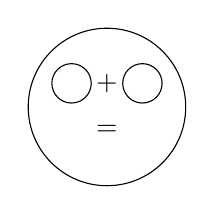
\begin{tikzpicture}
\draw (0,0) circle (1);
\draw (-0.45,0.3) circle (0.25);
\node at (0,0.3){$+$};
\draw (+0.45,0.3) circle (0.25);
\node at (0,-0.3){$=$};
\end{tikzpicture}\\
Cas particulier bien connu 0+0=0
\end{center}
A partir de $0$,  il construit l'ensemble des entiers relatifs :
$$\begin{aligned}
2+(2-4)&=&(2+2)-4&=&0\\
2+(1-3)&=&(2+1)-3&=&0\\
2+(0-2)&=&(2+0)-2&=&0\\
\end{aligned}$$
Ainsi "en supprimant le zéro" dans le membre de gauche, l'égalité devient 
$$2+(-2)=0.$$
le nombre négatif $-2$ "naît" et il l'\impo{opposé} de 2 .\\ 
Dans le supérieur, nous rencontrons de nombreux ensembles : les entiers naturels, les entiers relatifs, les fractions, les réels, les complexes, les polynômes, les vecteurs, les matrices, les fonctions continues etc.  L'objectif de ce cours est de suivre le cheminement de l'enfant en généralisant à un ensemble  $A$  quelconque et non plus l'ensemble des entiers. 
Comme un enfant aimant additionner et multiplier, un Mathématicien souhaite structurer un ensemble avec des opérations appelées \impo{lois de composition} qu'il appelle une \impo{structure algébrique}. L'addition et la multiplication  obéissent à plusieurs propriétés algébriques : l'associativité et la commutativité. De nombreuses structures algébriques étudiées obéissent à certaines, mais pas nécessairement à toutes, de ces lois. $0$ est un élément particulier de l'addition appelé l'\impo{élément neutre} c'est à dire il laissent tous les autres éléments inchangés lorsqu'il est composé avec eux. On se posera la question d'existence et d'unicité de l'élément neutre. La notion d'\impo{élément symétrique} généralise le concept d'opposé en rapport avec l'addition.\\
 
\end{Texte}


\section{Lois de compositions}
\begin{Definition}[Loi de composition interne]
Soit $A$ un ensemble.\\
Une \defi{loi de composition interne}, $\bigtriangleup$, est une application qui, à deux éléments de $A$, associe un élément de $A$ :
$$ \Fonction{\bigtriangleup}{A\times A}{A}{(x,y)}{x \bigtriangleup y}.$$
\end{Definition}
\begin{Exemple}
\begin{itemize}
\item Sur $\R$, l'addition définie par $\Fonction{+}{\R\times \R}{\R}{(x,y)}{x + y}$, la soustraction $\Fonction{-}{\R\times \R}{\R}{(x,y)}{x - y}$ et la multiplication $\Fonction{-}{\R\times \R}{\R}{(x,y)}{x \times y}$ sont des lois de composition internes.
\item Sur $\N$, la soustraction n'est pas une loi interne, mais elle l'est dans $\Z$.
\item Sur $\N^*$,  l'exponentiation définie par $\Fonction{}{\N^*\times\N^*}{\N^*}{(a,b)}{a^b}$, le PGCD ou le PPCM sont des lois internes.
\item Soit $X$ un ensemble. Sur l'ensemble des parties de $X$, $\mathcal{P}(X)$, l'union définie par $\Fonction{\cup}{\mathcal{P}(X)\times \mathcal{P}(X)}{\mathcal{P}(X)}{(A,B)}{A \cup B}$ et l'intersection $\Fonction{\cap}{\mathcal{P}(X)\times \mathcal{P}(X)}{\mathcal{P}(X)}{(A,B)}{A \cap B}$ sont des lois de composition internes.
\end{itemize}
\end{Exemple}

\begin{Definition}[Loi de composition externe] 
Soit $X$ et $A$ deux ensembles.\\
Une \defi{loi de composition externe}, $.$, est une application qui, à un élément de $X$ et un élément de $A$, associe un élément de $A$ :
$$ \Fonction{.}{X\times A}{A}{(\lambda,x)}{\lambda. x} $$
\end{Definition}
\begin{Exemple}[\((\R^2,.)\)]
La multiplication par un scalaire sur l'ensemble des vecteurs du plan  $\R^2$ définie par 
$$ \Fonction{.}{\R\times\R^2}{\R^2}{(\lambda,(x_1,x_2))}{(\lambda.x_1, \lambda.x_2)}.$$ est une loi de composition externe.
\end{Exemple}

\section{Propriétés éventuelles des lois de composition interne}
\begin{Definition}[Commutativité et associativité]
$\bigtriangleup$ est
\begin{enumerate}
\item  \defi{associative} : si $\in(x,y,z)\in A^3$, $x \bigtriangleup (y \bigtriangleup z) = (x \bigtriangleup y) \bigtriangleup z$.
  On ne considèrera que des loi associatives.
\item
 \defi{commutative} : si $\forall(x,y)\in A^2$, $x \bigtriangleup y = y \bigtriangleup x$.
 \end{enumerate}
\end{Definition} 
 \begin{Exemple}
\begin{itemize}
\item Sur $\R$, l'addition et la multiplication sont commutatives et associatives. Ce n'est pas le cas de la soustraction car $1-0\neq 0-1$ et $1-(2-3)=2\neq -4= (1-2)-3.$
\item Sur $\N^*$,  l'exponentiation n'est pas commutative $1^2=1\neq 2=2^1$ et non plus associative $\left(2^2\right)^3 = 64\neq 256 =2^{(2^3)}$.
\item Sur  $\mathcal{P}(X)$, l'union et l'intersection sont commutatives et associatives.
\end{itemize}
\end{Exemple}
\begin{Remarque}
Quand la loi est associative, la \defi{notation itérée} est
\begin{itemize}
\item en cas d'une loi de multiplication : $\forall a\in A,\forall n\in\N^*: x^n=\overbrace{x\times \dots \times x }^{\text{n fois}} $
\item en cas d'une loi d'addition : $\forall a\in A,\forall n\in\N^*: nx=\overbrace{x+ \dots + x }^{\text{n fois}} $.
\end{itemize}  
\end{Remarque}

\begin{Definition}[Distributivité d'une loi sur une autre]
Soit $A$ un ensemble et $\bigtriangleup$ et $\square$ deux lois de composition internes sur $A$.\\
On dit que $\bigtriangleup$ est \defi{distributive} sur $\square$ si:
$$ \forall x, y, z  \in A :\quad   x \bigtriangleup (y \square z) = (x \bigtriangleup y) \square (x \bigtriangleup z)\text{ et }(y \square z) \bigtriangleup x = (y \bigtriangleup x) \square (z \bigtriangleup x).$$
\end{Definition} 
\begin{Exemple}
\begin{itemize}
\item Sur $\R$, la multiplication est distributive sur l'addition mais l'addition n'est pas distributive sur la multiplication car $1+(2\times3)=7\neq 5=1\times 2+ 1\times 3$.
\item Sur  $\mathcal{P}(X)$, l'union et l'intersection sont distributives l'une par rapport à l'autre.
\end{itemize}
\end{Exemple}
\section{Élément neutre et symétrique}
\begin{Definition}[Elément neutre]
$\bigtriangleup$ admet \defi{un élément neutre} si il existe $ e\in A$ tel que $\forall x\in A$, $x \bigtriangleup e = e \bigtriangleup x = x$.
\end{Definition}
\begin{Proposition}[Unicité de l'élément neutre]
Si $\bigtriangleup$ admet un élément neutre, alors celui-ci est unique.
\end{Proposition}
\begin{Demonstration}
Supposons qu'il existe deux éléments neutres $ e$ et $e'$.\\
On a $e \bigtriangleup e'\overbrace{=}^{e \text{ elt neutre}}e'$ et $e \bigtriangleup e'\overbrace{=}^{e' \text{ elt neutre}}e$. Ainsi $ e=e'$.
\end{Demonstration}
\begin{Exemple}
\begin{itemize}
\item Sur $\R$, $1$ est l'élément neutre de la multiplication et $0$ de l'addition.
\item Sur  $\mathcal{P}(X)$, l'ensemble vide $\emptyset$ est l'élément neutre de l'union et  $X$ de  l'intersection.
\end{itemize}
\end{Exemple}

\begin{Definition}[Élément symétrique et loi symétrique]
Soit $ x\in A$ et la loi $\bigtriangleup$  admettant  un élément neutre $e$ .\\
$x$ admet un \defi{symétrique} pour $\bigtriangleup$ si il existe $x'\in A$ tel que $x \bigtriangleup x' = x' \bigtriangleup x = e$. Dans ce cas, $x'$ est appelé le \defi{symétrique} de $x$.
\end{Definition}
\begin{Proposition}[Unicité de l'élément symétrique]
Soit $\bigtriangleup$ une loi associative et admettant  un élément neutre $e$.\\
Si $x$ admet un symétrique $x'$, alors celui-ci est unique.
\end{Proposition}
\begin{Demonstration}
Supposons qu'il existe deux éléments symétriques $x'$ et $x''$.\\
On a $(x' \bigtriangleup x)\bigtriangleup x''=e\bigtriangleup x''=x''$ et $(x' \bigtriangleup x)\bigtriangleup x''\overbrace{=}^{\bigtriangleup \text{ associative}} x'\bigtriangleup(x\bigtriangleup x'')=x'\bigtriangleup e=x'$.  Ainsi $x'=x''$.
\end{Demonstration}
\begin{Vocabulaire}
Le symétrique est appelé :
\begin{itemize}
\item \defi{opposé} en cas d'une loi additive $+$
\item \defi{inverse} en cas d'une loi multiplicative $\times$
\end{itemize}
\end{Vocabulaire}

\begin{Exemple}
Sur $\R$,  l'inverse de la multiplication d'un réel non nul $x$ est $\frac{1}{x}$ et l'opposé de l'addition d'un réel $x$ est $-x$.
\end{Exemple}

\begin{Definition}[Loi symétrique]
La loi $\bigtriangleup$ est  \defi{symétrique} si la loi est associative et si tout élément de $A$ admet un symétrique.
\end{Definition}

\begin{Exemple}
Sur $\R$, la multiplication n'est pas inversible car $0$ n'a pas d'inverse. En revanche sur $\R^*$, la multiplication est inversible.
\end{Exemple}
\section{Parties stables}
\begin{Definition}[Partie stable]
Soit $B$ une partie non vide de $A$.\\
$B$ est \defi{stable} pour $\bigtriangleup$ si  
$$\forall x, y \in B :\quad   x \bigtriangleup y \in B.$$
\end{Definition}
\begin{Exemple}
\begin{itemize}
\item Sur $\R$, les ensembles $\Q$, $\Z$, $\N$ et les nombres pairs sont stables pour l'addition. 
\item Sur $\C$, l'ensemble $ \mathcal{U}$ des nombres complexes de module 1 est stable pour la multiplication car le produit de deux nombres
complexes de module 1 est un nombre complexe de module 1.
\end{itemize}
\end{Exemple}
\begin{Definition}[Loi induite]
Soit $\bigtriangleup$ une loi sur $A$ et $B$ une partie de $A$ stable pour $\bigtriangleup$.\\
La \defi{loi induite $\tilde{\bigtriangleup}$} est définie par  :
$$ \Fonction{\tilde{\bigtriangleup}}{B\times B}{B}{(x,y)}{x \bigtriangleup y}.$$
Pour alléger les notations, on identifie $\tilde{\bigtriangleup}$ à $\bigtriangleup$. 
\end{Definition}
\begin{Exemple}On munit  l'ensemble $ \mathcal{U}$ des nombres complexes de module 1 avec la loi induite $*$ sur $\C$.
\end{Exemple}









\end{document}
